% !TEX TS-program = pdflatex
% !TEX encoding = UTF-8 Unicode

% for a word count:
%https://app.uio.no/ifi/texcount/online.php

% This is a simple template for a LaTeX document using the "article" class.
% See "book", "report", "letter" for other types of document.

\documentclass[hidelinks,11pt]{article} % use larger type; default would be 10pt


\usepackage[utf8]{inputenc} % set input encoding (not needed with XeLaTeX)
\usepackage[backend=biber, style=authoryear]{biblatex}

% basic bib file
%\addbibresource{bibliography.bib}
% by lit type
\addbibresource{../bib/software.bib}
\addbibresource{../bib/data.bib}
\addbibresource{../Literature_Review/Literature/OSM_Quality/osm_quality.bib}
\addbibresource{../Literature_Review/Literature/Past_Similar_Work/related_work.bib}
\addbibresource{../Literature_Review/Literature/Network_Analysis/network_lit.bib}
\addbibresource{../Literature_Review/Literature/Bicycling/general_cycling.bib}


%%% Examples of Article customizations
% These packages are optional, depending whether you want the features they provide.
% See the LaTeX Companion or other references for full information.

%%% PAGE DIMENSIONS
\usepackage{geometry} % to change the page dimensions
\geometry{a4paper} % or letterpaper (US) or a5paper or....
% \geometry{margin=2in} % for example, change the margins to 2 inches all round
% \geometry{landscape} % set up the page for landscape
%   read geometry.pdf for detailed page layout information

%\usepackage{graphicx} % support the \includegraphics command and options

\usepackage[parfill]{parskip} % Activate to begin paragraphs with an empty line rather than an indent

%%% PACKAGES
\usepackage{hyperref}
\usepackage{booktabs} % for much better looking tables
\usepackage{array} % for better arrays (eg matrices) in maths
\usepackage{paralist} % very flexible & customisable lists (eg. enumerate/itemize, etc.)
\usepackage{verbatim} % adds environment for commenting out blocks of text & for better verbatim
%\usepackage{subfig} % make it possible to include more than one captioned figure/table in a single float
\usepackage{graphicx}
\graphicspath{{../images/}}
\usepackage{caption}
%\usepackage{subcaption}
\usepackage{multirow} % allows multiple rows per cell
% These packages are all incorporated in the memoir class to one degree or another...

%%% HEADERS & FOOTERS
\usepackage{fancyhdr} % This should be set AFTER setting up the page geometry
\pagestyle{fancy} % options: empty , plain , fancy
\renewcommand{\headrulewidth}{0pt} % customise the layout...
\lhead{}\chead{}\rhead{}
\lfoot{}\cfoot{\thepage}\rfoot{}

%%% SECTION TITLE APPEARANCE
\usepackage{sectsty}
\allsectionsfont{\sffamily\mdseries\upshape} % (See the fntguide.pdf for font help)
% (This matches ConTeXt defaults)

%%% ToC (table of contents) APPEARANCE
\usepackage[nottoc,notlof,notlot]{tocbibind} % Put the bibliography in the ToC
\usepackage[titles]{tocloft} % Alter the style of the Table of Contents
\renewcommand{\cftsecfont}{\rmfamily\mdseries\upshape}
\renewcommand{\cftsecpagefont}{\rmfamily\mdseries\upshape} % No bold!

%%% END Article customizations

%%% The "real" document content comes below...


\title{The Suitability of Open Street Map Data for Defining and Assessing Urban Bicycle Networks}
\author{Hugh Kelley}
%\date{} % Activate to display a given date or no date (if empty),
         % otherwise the current date is printed 

%%%% word counts
% 19 aug noon: 8,128


\begin{document}
\maketitle

\pagebreak


Name: Hugh Kelley

Programme: MSc. Smart Cities and Urban Analytics

Institution: University College London

Date:

Word Count:

This dissertation is submitted in partial fulfillment of the requirements for the degree of Master of Science in Smart Cities \& Urban Analytics from University College London.

I, Hugh Kelley, confirm that the work presented herein is my own. Where information has been derived from other sources, I confirm that this has been indicated.
\pagebreak

All maps displayed herein use data from OpenStreetMap 2019 and from the Crown Ordnance Survey 2019.

\medskip
 
All maps are projected in UTM-30 EPSG:322300.

\pagebreak

acknowledgements.\\

Thank you to all the people who helped me write this dissertation! 

\pagebreak

\section{Abstract}
text

\pagebreak

\tableofcontents
\pagebreak

\listoffigures
\pagebreak

\listoftables
\pagebreak

\section{Introduction}

	%777 words


\begin{quote}
``When you get these incomplete networks you have this situation where great, you have this fresh new bike lane, you're excited you know?'' Maerowitz said. ``This infrastructure is working for you and then suddenly it's gone and you have to go back out into traffic again.'' - \cite{juhasz2019}.
\end{quote}
 
\subsection{The Challenge of Cycling in Cities}

What makes a city comfortable for cycling? The conditions are obvious when one sees them, but defining the characteristics quantitatively is challenging. More than half of the world's population lives in cities\parencite{half}. Cycling is of obvious importance to the well-being of the world's  urban population in terms of the macro-climate crisis, local pollution problems,  public health, wealth disparities, and urban traffic congestion. A commonly researched question is ``What factors have the most significant effect on cycling rates?'' Only recently, however, have researchers begun to study cycling from a network perspective. A comprehensive understanding of cycling networks is hindered by multiple challenges. 

%One is access to and the existence of necessary data. Another is the availability of tools for constructing data into a representational network and assessing that that network, which are only beginning to emerge.   

First is the scope of the analysis, considering individual changes to roads instead of the status of the entire transportation network from the cyclist's perspective.  The majority of work on this question approaches the matter from a perspective of discrete policy intervention and the effect of marginal improvements on cycling. This approach fails to build a comprehensive theory of cycling rates that a network analysis approach can offer. Only a network approach can offer a complete understanding of the level of service for cyclists in a community. 

The second consideration is the difficulty of obtaining data used by the studies that do take a comprehensive network approach. The most successful study used high quality data regarding street characteristics that the authors obtained from the local government. In many situations for financial or political reasons this data may not be available. This dissertation therefore uses open data to replicate the methods of previous work. 

%Basic attitude is that improvements to infrastructure only matter to the extent that they improve safe connectivity to ``important'' nodes/edges.  The implication of this view is that infrastructure changes are unlikely to have a meaningful effect on behavior in the system until a critical mass or tipping point is reached in the network. 

In this context, this dissertation contributes to the understanding of cycling infrastructure and cycling behavior by using London as a case study. London is an attractive case because it has a considerable cycling population but does not yet have the level of infrastructure that exists in world leading cities like Copenhagen \parencite{mayor}. Thus London's position at a mid-point of cycling infrastructure development allows for the identification of strengths and weaknesses to a live program of improvement.


%%%%%%%%%%%%%%%%%%%%%%%%%%%%%%%%%%%%%%%%%%%%%%%%%%%%%%%%%%%%%%%%%%%%%%%%%%%%%%%%%%%%%%%%%%%%%%%%
\subsection{Research Question}
%
%\subsection{Key Questions}
%what was the scope and how was it defined \\
%How well does Open Street Map serve as a data source \\
%what filters/networks were used \\
%what are reasonable walking and cycling speeds \\
%what were the travel times calculated \\
%what was the directness of travel on different networks \\
%what is the distribution of travel times in the different networks \\
%How does transit by public transport compare to cycling? \\
%what lsoas changed the most and least across networks \\
%how did removing road types affect the number of lsoa centers connected? \\
%how long did the calculations take? \\
%Did removing directionality mediate the effect of removing streets? \\


The goal of this dissertation is to build and interpret quantitative measures for the quality of London's cycling network. First, OpenStreetMap data will be assessed as the primary data source for building representations of London's cycling infrastructure. Second, metrics will be calculated and compared for the different network representations. Third the comparisons will be used as the basis for drawing conclusions about the London cycling infrastructure network. The most important objective of this dissertation is to specify how data and methods can be combined and improved to provide for a fuller understanding of the current quality of the networks and to indicate the best ways to improve the network in the future. 

The dissertation will address a few secondary questions. First, to what extent is transportation space in London a zero sum game? Does improving the experience of cyclists require taking space from motorists? Second, are there any key differences between the grid-like networks studied in past research in North American Cities and the more tree-like network of London streets? 

%This research intends to define the overall suitability of a city to cycling using estimates of roads cyclist are and are not willing to use and the effect these decision have on travel times. The central research question is: \textit{how does a preference for safety decrease accessibility in central London when traveling by bicycle?} It extends the literature in three ways; extending quantitative research to a holistic approach rather than focusing on individual edges or nodes, extending holistic approaches to quantitative outcomes rather than visual or anecdotal conclusions, and by emphasizing the use of open source tools and data that are available to any member of community. 
%
%The research provides a methodology that allows a community to identify nodes and edges for improvement that will have the largest impact on the overall network, quantify the expected improvement, and thus require from elected officials specific changes to the roads in their communities.  
%
%The issue implied by these research questions is: to what extent is street level transportation space a zero-sum game? 
%
%Can a high level of service for cyclists be built without taking large amounts of important space away from automobile traffic? 
%
%The intended outcomes of this research include(1) an understanding of the roles of location and connectivity for cycling infrastructure and (2) an understanding of the usefulness of Open Street Map data for estimating these sorts of measures. 

\subsection{Ethical Risks}

This project relies entirely on publicly accessible data. For this reason, ethical risks are not present in the research methodology.  

\subsection{Research Structure}

First, existing work on this research area will be reviewed and the techniques to be built upon will be identified in section \ref{literature}.  Then  section \ref{methods} will describe a general methodology for defining the strength of cycling infrastructure in a city. Section \ref{data} will describe the data available regarding London's cycling infrastructure in the context of past work, and what is available for other cities and through other channels that were not available to this research. The steps taken for data cleaning, transformation and joining will be specified. Section \ref{analysis} will describe the implementation of this methodology for London, identifying the scope of the case study, defining the exact data collected and transformed and the specific tools used, and reporting the results of the implementation. Finally section \ref{conclusions} will set forth conclusions, identify opportunities to improve the methodology and the quality of the data, and make key recommendations for further improving the London cycling infrastructure network. 

After critically reviewing this existing research, a methodology for using open source tools and data to estimate the relative strength of a cycle network and a method for prioritizing improvements will be specified.

The review that follows takes an initial look at typical literature considering how to promote cycling, recent attempts to use network analysis to accomplish this same goal, and closes with a look at work analyzing data sources relevant to this investigation. 

%\subsection{The role of the researcher}
%
%Read other versions of this and see if it makes sense for this 




\section{Literature}

	% 2435 words


\subsection{Cycling Behavior}

The most important conclusions from literature that tries to predict cycling behavior is the focus on multiple types of cyclists, and the factors that influence each type's decision to cycle. Most often, four types of cyclists are used, ``strong and fearless'', ``enthused and confident'', ``interested but concerned'', and ``no way no how'' (\cite{dill2013four}). This categorization is sometimes changed to so that the final category is dedicated to children with their set of safety requirements for a suitable cycling environment (\cite{mekuria2012low}). The literature separates the decision to cycle into the decision of cycling frequency, how often someone who is willing to cycle generally chooses to do so, and the decision to cycle at all, with different factors influencing each decision (\cite{stinson2005comparison}). 

Despite behavioral differences between these categories, research has shown that all cyclists are willing to sacrifice time and energy for increased safety on their route\cite{winters2011motivators}. Indeed, psychological research showed that fear is a significant factor during an urban cycling trip (\cite{ellett2018state}). This is important given the sensitivity cyclists show to efficiency (\cite{wuerzer2015cycling}). The impact of a route change can be very significant, for instance a higher frequency of stop signs on a route can double the energy required for a journey (\cite{fajans2001bicyclists}). Given the common trade off between efficiency and safety, it was found that the effect of infrastructure improvements is very dependent on context, effect is a function of the change in safety, and the importance of the location to trips (\cite{kondo2018bike}), improvements that meaningfully increase safety at important locations have the largest effect. 

Several studies looked at the importance of perception in behavior change, assuming that a real change in safety is irrelevant if it is not perceived by potential cyclists as a change(\cite{li2012physical} and \cite{parkin2007models}). This gives rise to literature that focuses on a behavior and attitude change approach from psychology the prioritizes change in habits and perception over infrastructure, with changes to the built environment only used where required to change perception (\cite{savan2017integrated}). This should be considered in the context of research showing that cyclist perceptions of danger are generally accurate (\cite{vandenbulcke2014predicting}). Thus it seems reasonable to conclude that despite the decision to cycle being a fairly complex mix of factors, the decision for almost any urban commuter, comes down to safety, and efficiency. An efficient network of safe edges, connecting important nodes, would be expected to have a meaningful effect on the rate of cycling in an urban area.  


%%%%%%%%%%%%%%%%%%%%%%%%%%%%%%%%%%%%%%%%%%%%%%%%%%%%%%%%%%%%%%%%%%%%%%%%%%%%
%%%%%%%%%%%%%%%%%%%%%%%%%%%%%%%%%%%%%%%%%%%%%%%%%%%%%%%%%%%%%%%%%%%%%%%%%%%%
\subsection{Cycling Networks}

\cite{buehler2016bikeway} is a very useful introduction to the literature on cycling networks. Unfortunately it concludes that very little true network analysis has been developed for cycle networks. The majority of papers they found could be categorized into those that focus exclusively on nodes, and those that focus on edges of the dual graph, where intersections are nodes and streets are edges. At the time of writing there were 115 papers citing Buehler's review, however all but 5 of them fail to take Buehler's central recommendation that \textit{If individual characteristics of a network's links and nodes contribute to cycling levels, it logically follows that a network of such features would as well...}. The ``Toward Studying the Whole Bicycling Network'' section of Buehler's review is a good overview of attempts up to 2016. The key findings were that continuity and connectivity of infrastructure is valued by cyclists. Of particular interest is the \cite{schoner2014missing} study of the relationship between network characteristics and cycling mode share in 74 US cities. That study found density of the network had the highest elasticity for effect on cycling rate. 

Several of the works reviewed contribute new ways of measuring ``quality'' of the infrastructure, these quality measures include a Bicycle Compatibility Index (BCI) (\cite{klobucar2007network}),  Bicycle Level of Service (BLOS) (\cite{lowry2012assessment}), and Level of Traffic Stress (LTS) (\cite{mekuria2012low}). Each of these can reasonably be viewed as an attempt to measure the ``safety'' of a network link. These studies generally lacked a rigorous method for prioritizing nodes by importance or defining a sample set of trips between nodes. Improvements to this will be addressed in the section reviewing network analysis literature. 

Buehler notes that a key challenge to using the network methods reviewed is data availability, this research hopes that network analysis can be a method for reducing rather than extending the amount of data necessary to understand a cycle network, as network statistics could be used to replace some empirical measurements as discussed below.  They further criticize the approaches as lacking empirical validation. Gathering accurate cycle traffic data and safety data is an immense challenge as demonstrated by the flow estimation techniques of \cite{gosse2014estimating} and the safety estimate techniques of \cite{puchades2018role}, which focuses on near misses as a proxy for predicting actual safety incidents, but acknowledges the difficulty of collecting near miss data without human observation. 

Since the publication of Buehler's review, the papers extending the full network analysis method have had moderate success. \cite{akbarzadeh2018designing} uses taxi trip data to weight the links between destinations in order to build communities of nodes that tend to be origin and destination pairs. While this is a novel approach to prioritizing edges, taxi usage tends to be for less frequent travel between nodes and the general literature as well as this work focuses on daily commuting, which is rarely accomplished by taxi. \cite{boisjoly2019bicycle} focuses on the directness of routes on cycle paths between nodes. 

\cite{doorley2019designing} focus on building cycle infrastructure to maximize a function of travel costs, infrastructure costs, health, traffic accidents, and pollution. While this is an interesting approach, it addresses a more political question in the sense that the key result of the algorithm is to recommend a specific amount of investment in cycle infrastructure to maximize the costs and benefits to all road users, The author's fail to recognize the prioritizing the goals of public policy is a normative and subjective exercise and that a model designed to give an ``objective'' answer to this question inherently reflects the author's preferences and when calibrated to ``the real world'' reflects the biases and preferences of the status quo, rather than the true ideal outcomes preferred by a population. Instead, modeling, especially for urban planning purposes, should accept an exogenous goal and implement it as efficiently as possible. For instance, cycle infrastructure, is explicitly intended to reduce motor vehicle use, it would make no sense to then use a model that determines the efficient level of motor vehicle use, the political process has already determined the answer and merely asks for implementation recommendations from the modeler. 

\cite{mauttone2017bicycle} similarly focuses on an optimization framework for cycling networks, choosing a subset of streets that are ``suitable to building cycle infrastructure''. This is odd in the sense that the goal of building cycle infrastructure is to \textit{create} streets that are suitable for cycling, not merely identify them. Similar to \cite{doorley2019designing}, they identify a cost to building cycle paths which they seek to balance against the benefits. 

Overall, it is not clear that a model for building cycle paths should be particularly cost sensitive. \cite{gu2017cost} found a very high return on investment to the budget for cycling infrastructure in New York City. The very idea of using network analysis for the development of cycle networks emphasizes the potential non linearity of the effect of building more infrastructure, with usage accelerating as the network approaches ``completeness'' in some for. In addition, cities tend to combine cycle infrastructure improvement with other required improvement and maintenance activities, mitigating the costs by being opportunistic in implementation. 

Lastly, \cite{osama2017models} uses a number of predictors including network statistics to predict bike travel within zones of Vancouver similar to \cite{schoner2014missing}. They found a positive coefficient for the density of the bike network in the zone. 

Thus while network analysis has been applied to cycle infrastructure, clearly there is not a consensus on the methodology. In particular, a definition of ``quality'' or ``safety'' has not been established. Additionally, a method for exploring the network of infrastructure defined is still lacking. 

The most direct inspiration for this work comes from \cite{furth2016network}. That anaysis built representations of the San Jose cycle network for different types of users using data collected and maintained by the local government. Data used included the locations of cycle tracks and shared paths, the width of street lanes, the width of bike lanes on those streets,  the volume of traffic by lane for each street, right of way in intersections and the structure of each intersection, and the frequency of bike lane blockages for each street. Futh then computes a "connectivity ratio" that is essentially the percentage of commuter trips from journey to work data that are possible for a given representation of the network. 

Furth notes that ``These connectivity methods do not necessarily require use of the LTS classification scheme. They can be applied with any classification scheme that distinguishes high- and low-stress segments.'' This is a vital component of this work as the majority of data that Furth uses is not available for London. In the methodology section, a process for building similar networks using data from Open street map will be specified. Furth also notes the computational burden of the analysis as a limiting factor. 

The second important inspiration for this work is \cite{boisjoly2019bicycle}. This work used a survey of cyclists route choices between sets of destinations in Montreal to estimate the probable path for a larger set of destinations. With these paths, they estimated the average directness of a journey in the city to identify neighborhoods with relatively low diretness of cycling routes.  Their analysis considered for a given route the percentage of the routes distance that occured on cycling infrastructure and the directness of the route relative to the directness of the shortest possible route between the given origin and destination. The routes were predicted using data from a survey of 1525 cyclists, which collected data on their cycle trips with regard to usage of bicycling infrastructure. the study specified a cost function that allowed for the expression of stress and distance in common units by penalizing high stress edges, increasing their distance cost, and reducing the distance cost of low stress edges. The cost function was estimated from the survey of cyclists. It is simply a measurement of how far from the shortest path the cyclist diverted in order to use a piece of cycling infrastrucucture. 

The strength of the boisjoly study is that it does not require high detail data on the street network, only the simple street connectivity network and data on the location of cycling infrastructure. The weakness of the study is twofold. It requires substantial survey data on route choice from network users and it uses minimal descrimination acros the quality of cycle infrastructure, and across the level of stress for a given street. 

``there is often a tradeoff between route directness and quality of route'' (\cite{boisjoly2019bicycle}). 

\subsection{Open Street Map Data Quality}

A central research question of this work is "how sufficient is Open Street Map (OSM) data for replicating the studies considered above," both of which rely on data unavailable for london, cycling route choice survey data and high detail street characteristic data. 

There is a strong body of existing research on the quality of OSM data. this can be divided into two focus areas and two types of methodology. The two focus areas are locational accuracy of features and the completeness of attribute tagging and description for features. the two methods for assessing this are extrinsic and intrinsic. Extrinsic uses an external dataset, usually professionally collected. The intrinsic analysis attempts to solely use an analysis of OSM data . 

Studies on locational accuracy are consistently extrinsic. For instance \cite{haklay2010good} compared Open Street Map in the UK to the government produced Ordnance Survey data for roads in the UK finding that there was about 24\% coverage of the UK and that features addd tended to be very close to their location in the Ordnance survey data. This is of minimal use to assessing cycle networks though because the characteristics of the features, streets, are of much more importance than their locations being highly precise. 

Assessing the accuracy and completness of feature attribute tagging in OSM is a more recent endeavor and more difficult due to the lower availability of data, the more frequently changing nature of the data as road works are undertaken and the very open structure of tagging of attributes in OSM.  

The use of OSM data for specialized routing applications has been considred by  \cite{mobasheri2017crowdsourced}. in this study, they considered the quality of sidewalk tagging in OSM from a number of cities for the purpose of routing wheelchair users. This study was looking for information about the surface type of pedestrian ways, the incline, and the width. They found found about 17\% coverage of sidwalks in Hamburg Germany and that coverage was best where density of features and tags was highest. This work combined extrinsic and intrinsic analysis of the question but did not take the opportunity to validate the intrinsic analysis with the extrinsic analysis. 

"Based on empirical results, it is concluded that OSM data of relatively large spatial extents inside all studied cities could be an acceptable region of interest to test and evaluate wheelchair routing and navigation services, as long as other data quality parameters such as positional accuracy and logical consistency are checked and proved to be acceptable."  

Hochmair wrote an article about the completeness of bicycle features in OSM. They used Google Maps to extrinsically validate the OSM data for bike trails in the US and Europe. while they found that coverage was fairly good but only considered fully separated bicycle infrastructure like segragated lanes and of-road trails, which is of limited use to the analysis of urban cycling networks where many cycling inrastructure features exist on shared roads. 

Finally \cite{zielstra2013assessing} considered the impact of bulk uploads of geospatial data to OSM. they found that in the United States, while government collected data had a higher level of completeness for motor vehicle related street network data, data for pedestrian related features was higher in OSM. This raises the possibility that for a well mapped area, OSM could be the best possible source of data for cycling, depending on the priorities of local governments in their data collectoin efforts. This is especially important in the context of the new Transport for London Cycling Infrastructure Database, which will be imported to OSM over the next few years \cite{tflcid}. Despite th possibility that there are meaningful problems with current cycle related ata in OSM today, OSM is likely to be the highest quality source of this data in the near future. 

Ultimately, the quality of OSM data for cycling related data is uncertain and the methodology and analysis will address an attempt to understand the quality levels in London, which it is thought will be at least as high as anywhere else in the world. 


\section{Methods}

	% 736 words


%%%%%%%%%%%%%%%%%%%%%%%
%- define scope, minimize area while capturing the largest number of trips by bicycle, trips in total, road casualties, and households and jobs. This will be some part of central London. 
%-- build boundary based on scope using postgis and qgis
%- define filters for OSM data
%-- this includes trying to understand the relationship between relations and individually tagged edges and nodes. 
%-- pictures of network, specific edges, and photos of real life infrastructure. 
%-build networks from data
%-- removing streets
%-- undirected
%- identify network nodes closest to lsoa centroids
%-compare \% of trips possible across Quant, bike 1, bike 2, and undirected versions. 
%- compare change in directness between bike 1 and bike 2.  
%-- compare bicycle accessibility to Quant
%-UTM-30 projection used as standard across all data. 
%%%%%%%%%%%%%%%%%%%5

\subsection{Scope}

The scope of the study will be defined to maximize the study's representation of London's cycling commutes, capturing as many trips by origin and destination as possible as well as considering the location of road casualties in London. This will be done in the context of the computing resources available, where travel time calculations for the origin destination matrix must be reasonable, less than one million pairs. 

\subsection{Defining Networks}

The first step in this investigation is to build a data set that represents the London cycling network as accurately as possible. This representation needs to reflect the fact that different cyclists are willing to use different streets as a function of the perceived safety of the street and the level of confidence of that cyclist. Thus, the data set will be multiple representations of the city cycling network that each represent a level of confidence, only including streets with a certain level of safety. 

A key question then is, how to quantify ``safety''. In a perfect world, this would be done empirically. This would involve a combination of cycle traffic volume collection, cycle traffic behavior observation, and interviews with a representative set of cyclists and non-cyclists about their decision making. All of this data could be compared to the cycling environment in different locations to find cyclist sensitivity to different factors. 

Networks will be defined as subsets of edges in the Open Street Map network. Open Street Map uses tags to associate street characteristics with the geometries that make up the map. Appendix XXXX contains the definitions from the OSM wiki page for each of the tags used.  

Using the network filters, the connectivity data is downloaded from OSM via the Overpass API as a JSON file. A graph is built with the nodes and ways from the Overpass data with edges coming from the ``way'' elements, and the nodes coming from the intersection of the edges as defined in OSM as well as the end of an edge. This requires simplification because the Open Street Map data includes many more nodes than just the endpoints and intersections. The network is simplified by removing nodes with degree 2, where the node simply connects one street to one other, unless there is a difference in directionality between them. That is, when a street changes from two way to one way, a node is placed at the intersection to denote that change.  Each of these steps can be accomplished using a combination of python packages OSMnx, (\cite{osmnx}) and Networkx (\cite{networkx}).

\subsection{Defining Origins and Destinations}
London was divided into 4765 Lower Super Output Areas (LSOA) for the 2011 census (\cite{lsoa}). One Origin/Destination (O/D) point will be selected for each LSOA in the scope. QUANT uses the node of highest degree in a given LSOA. For calculating a sample of routes on the networks, this analysis used the node closest to the centroid of each LSOA. 

\subsection{Assessing Networks}

A key point of interest is the network structures that result from different filters. For different filters, the count of nodes and edges, and therefore the overall density of the network will be considered. The size of the largest component will be considered as well as the number of O/D pairs connected by the network. 

The distance of the shortest path between each origin and destination will be calculated for each network with more than 50\% of pairs connected. These data will be converted to measures of directness, dividing by the straight-line distance between the two points, and into travel times, dividing by the speed of a cyclist as estimated by Google Maps. 

In addition to calculating the multi-directed graphs for different OSM filters, distances are calculated for undirected versions of the graph. This will be used to investigate how building infrastructure for cyclists to travel safely against traffic could further raise accessibility or replace the need to build infrastructure that takes space from other users on main roads. 

Finally, the mean and shape of the cycling distribution will be compared to the shape of the QUANT transport distribution.  



\section{Data}

	% 1335 words

\subsection{Open Street Map}

%Intro and overview

Open Street Map is a mapping project started in 2004 to collect volunteered geographic information. It consists of geometries drawn by users, either in person, as they travel through a city or remotely, looking at donated satelite images of cities. Open street map provides community generated geospatial data. This data is accessible via the overpass API from several hosts. Geoff Boeing describes using the OSM API query language as "notoriously difficult" (\cite{osmnx}). 


%Data Structure


Second to the actual geometry of a "way", streets and paths, node, single point on the map, or relation, collection of ways nodes and other relations are tags. Tags specify what a particular geometry is, what its characteristics are, and rules for use or other characteristics of the geometry. This allows for differentiation on the map between public and private areas, specification of what exactly a node is referencing, an intersection, mailbox, or a business location, or the type of traffic allowed or commonly seen on a street way. 


% Possible Problems with Data

As discussed in Literature reivew section XXXXXXX
 
 
 There are four possible problems with Open Street Map, missing geometries, inaccurate geometries, missing tags and inaccurate tags. The review of literature will provide detail on attempts to measure the accuracy of the data in Open Street Map.
 
 
% General Way to build data by filtering. 



Compare Relation = cycleway to a list of edges and nodes tagged cycleway

Adding living streets and residential streets don't do much. 

Part of the problem is the lack of consistent tagging, it only takes one line segment missing a tag to disconnect two nodes,

but this also reflects the fact that getting somewhere within London nearly always requires leaving cycle infrastructure at some point and using main roads. 

Two basic problems for using OSM data to define cycling networks were found. The first is that defining the network by relation exagerates the network, the second is that relying on the metadata tags of individual features understates the cycle network. Looking at OSM it is clear that the relations identifying bike routes are not reflecting sets of ways and nodes with a given tag, or reflecting streets and intersections where cycling is meaningfully safer than other streets and intersection. At the same time, it is clear that there are many ways and nodes that are more accomodating to cyclists than their OSM metadata indicates. 


Cite OSM wiki page
https://en.wikipedia.org/wiki/OpenStreetMap


%%%%%%%%
% image of OSM London cycle network by relation
% image of OSM London cycle network by tag
% image of OSM missing tag situation from Overpass turbo
% image of same location street view
% image of OSM implied cycle infrastructure
% image of real street without cycle infrastructure. 
%%%%%%%%%%%%%



In the case of the relation, Quietway XXX was examined in person. figure XXX shows an image of Brandon rd, a part of the quiet way. this way is tagged
Brandon rd is part of OSM relation XXX the Hackney Camden cycle route.  this road though, as can been seen in the image, has no actual cycle inrastructure. This in Open street map, it is tagged as an unclassified highway. There is a tag noting the max speed is 20 mph. Data collected for 20 mph streets found that as many as 80\% of drivers exceeded these limits. 
https://www.thesun.co.uk/news/7253694/20-mph-zones-cause-more-deaths/

In other cases, osm underestimates the quality of cycling infrastructure. for instance the intersection of Mile end Road and Cambridge Health Road in the borough of tower hamlets is a high traffic intersection both for automobiles and for cyclists. It is an integral part of the Stratford to Aldgate cycle super highway. This intersection has been reworked to be safer for cyclists. In open street map though, it i labeled a "trunk" highway, due to its high traffic nature. It is way 7058092014. There is also a tag cycleway:left=lane indicating that there is a cyclelane on the left side of the street. 

\cite{osm}

\subsection{A Close Look at an Open Street Map Case Study}

\begin{figure}
\centering
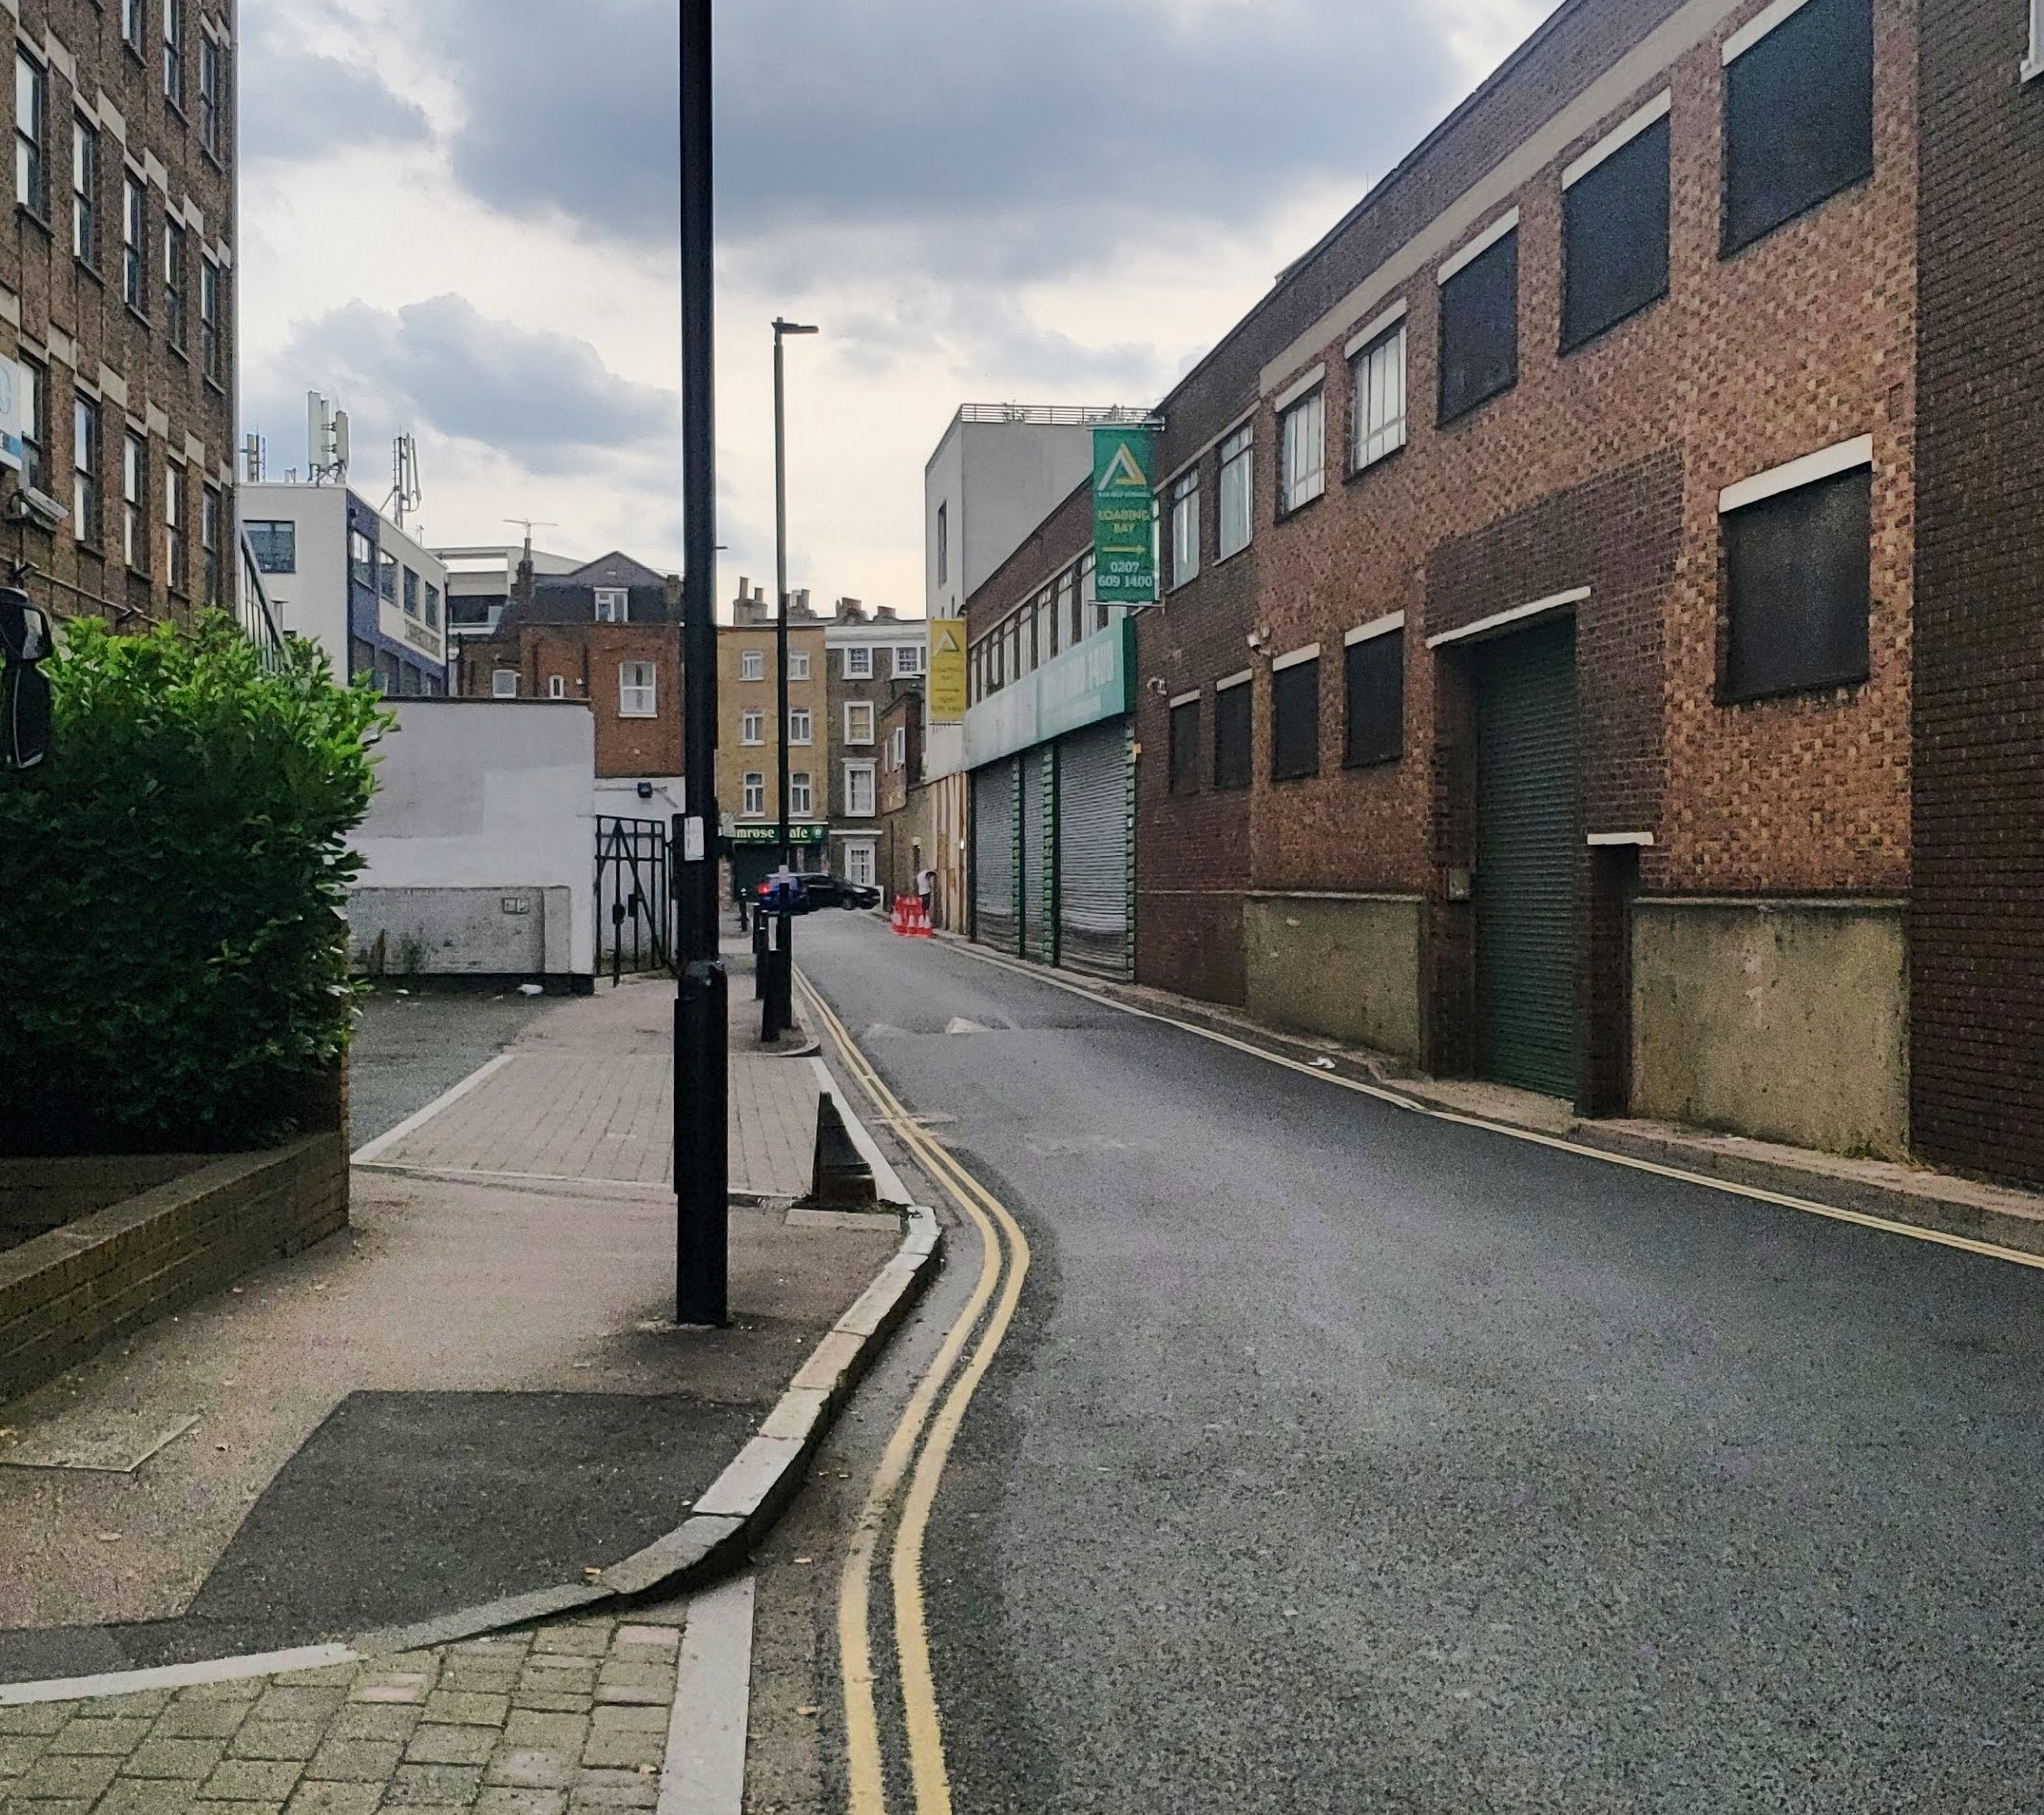
\includegraphics[width=0.6\textwidth]{brandon_rd_cropped}
\caption{image of quietway}
\end{figure}

\begin{figure}
\centering
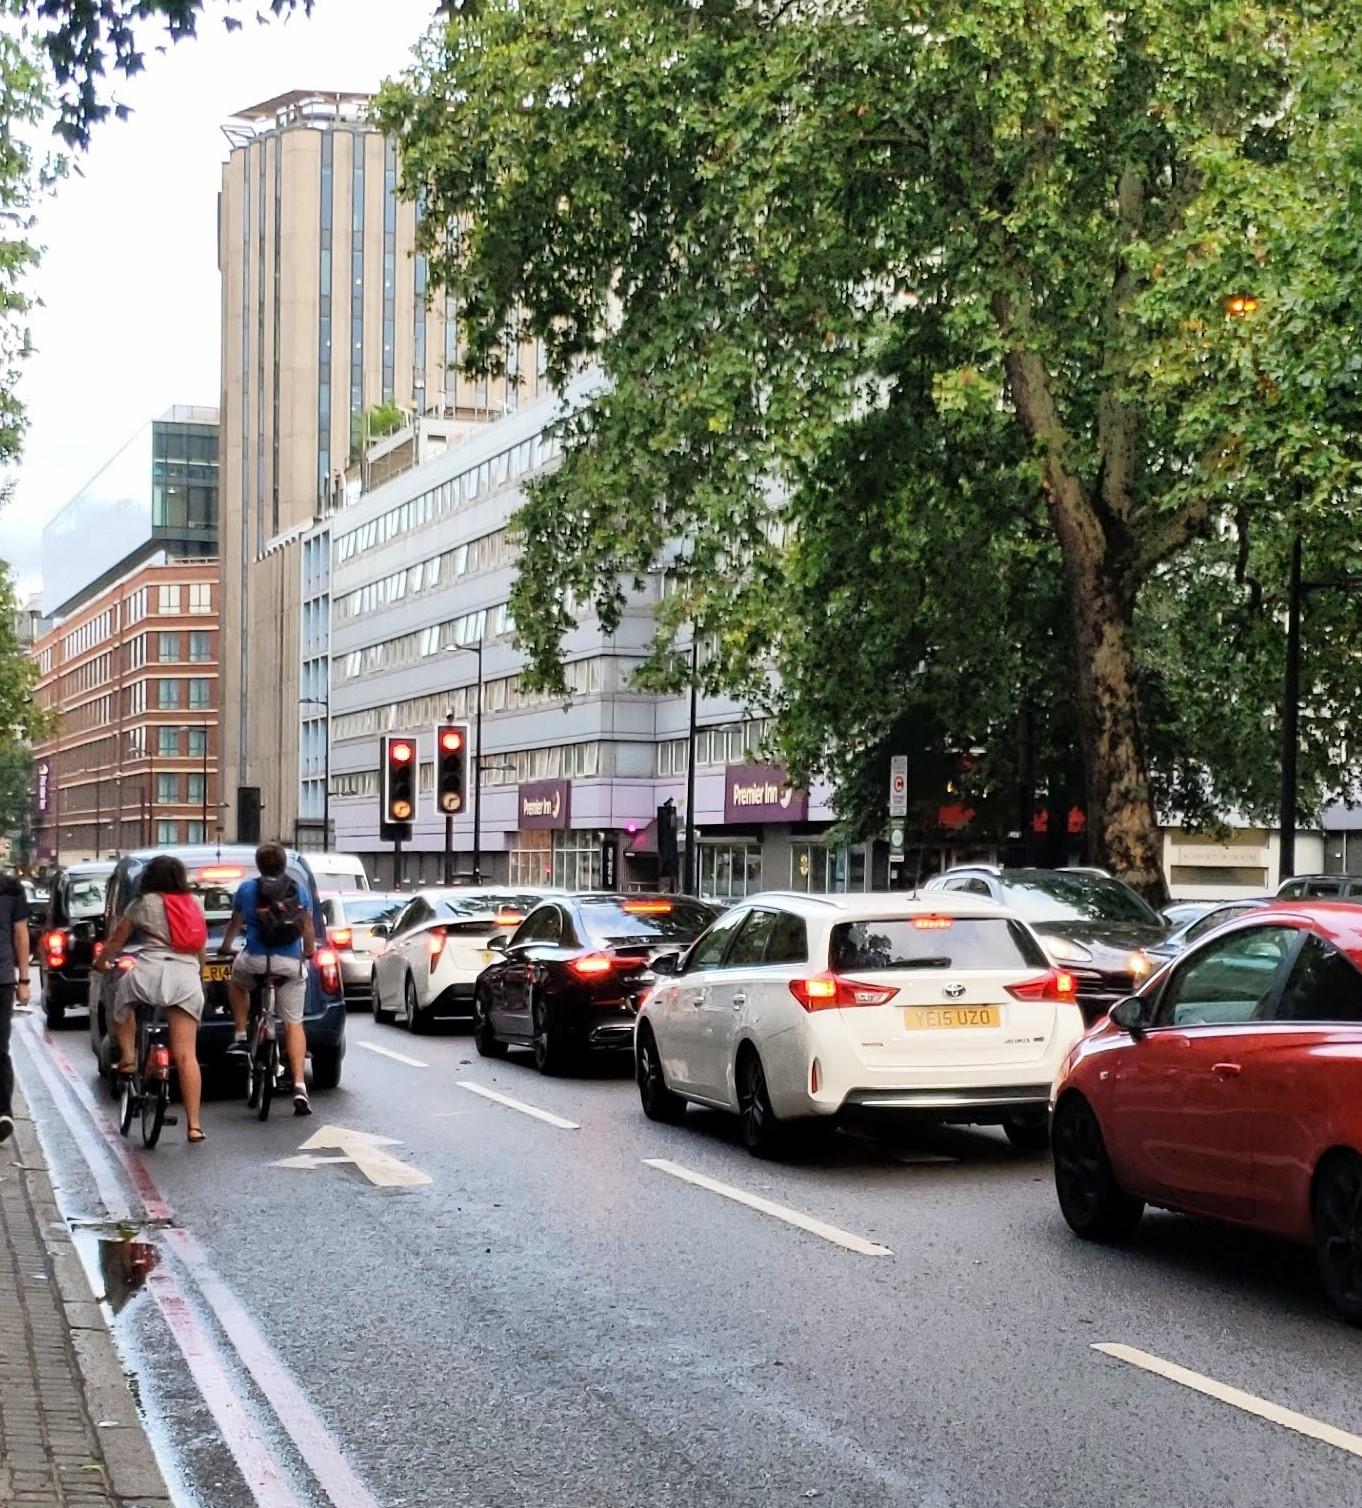
\includegraphics[width=0.6\textwidth]{euston_rd_cropped}
\caption{An image of Euston Road}
\label{fig:euston}
\end{figure}

\subsection{Transport for London Cycling Infrastructure Database}

\cite{tflcid}

This data was in the process of being publishing during the period of research for this work. While it was not available at the time of publication, it is notable because it promises to raise the quality and volume of OSM data for London substantially. It includes 2,000km of cycle lanes as well as hundreds of thousands of parking spaces, cycling related signs and other relevant features. \cite{osmtflcidwiki}. 

Section XXXX from the Lit Review addressed to possibility for bulk data uploads to dramatically enhance OSM data quality and this may be one example. The data was professionally surveyed. 

\subsection{QUANT}

The QUANT dataset of public transport travel times was .

CITE

The of 22 million pairs, 5.8 million pairs had no public transport link. To clean this data, the set is cut down to match the scope of the the investigation. Where there is no link between an origin destination pair, a link is constructed by combining the walking time from the origin to the node of highest degree in another LSOA where public transport is available to the destination LSOA. 

The walking speed used will be taken from google and the distance is the straight-line distance between two points. This is less accurate than actually finding the walking route between the two points but this level of detail was not computationally feasible. 

The QUANT data provides a point of comparison for cycling travel times to be calculated. 

\subsection{2011 Census Journey to work data}

The 2011 census asked each household where they lived, where they worked and how they traveled to work the preceding week (\cite{jtw}). Thus data for origin and destination by mode of transport was available. This data will be used to help define the optimal scope as well as to compute a ``connectivity ratio'' like that of \cite{furth2016network} for a network. 

This data is shared through the Nomis Labor Force website as multi-sheet excel pivot tables. Making the data usable required, stripping the meta data headings from each sheet, importing the book to pandas dataframe by sheet, melting from a pivot table to long data with origin, destination, and count columns, adding the sheet name that identified the mode of travel as a column, appending each individual sheet together into a single dataframe, and pushing the dataframe to the sql database. 

\subsection{LSOA boundaries and data}
	
LSOA boundaries were obtained from  \cite{lsoageoms}. The LSOA boundareis were determined as a part of the 2011 census containing approximately 5000 people each. These are used, first to specify a boundary for the scope of the study and then to specify origin and destination nodes on the network. The node closest to the centroid of each LSOA is selected as the origin and destination or that LSOA. Where LSOA's were comprised of multiple polygons, the centroid of the largest polygon was used. These polygons were used for the production of maps seen in the Analysis section XXXXX. 

On maps created using these boundaries the copyright must be stated. This is
%"Contains National Statistics data © Crown copyright and database right [2015]" and "Contains Ordnance Survey data © Crown copyright and database right [2015]"
	
\subsection{Road KSI data}

Data on those killed or seriously injured on London streets is available through CITE. This was used to assist in determining the scope of the investigation. While it was hoped that the data could be used to build an estimate of danger to cyclists on London's streets several obstacles prevented this. The first is the change in infrastructure over time and lack of data about the exact infrastructure present at the time and location of each incident. Second was the lack of high resolution data about cyclist volumes. An area that has a particularly high KSI rate may be especially dangerous or may be relatively safe after adjusted for cyclist miles traveled, an unknown. London has begun collecting some data on cyclist volumes although this remains fairly sparse. \cite{cyclistksi}
	
\subsection{Data import, storage, cleaning, and joining}

data import was done in python using the csv, pandas, geopandas, json, and osmnx packages. 
Data from OSM was converted from json to a dataframe, tags simplified, edges truncated, geometry simplified. 
Geometry was converted to well known text and multi-lines were broken into several single line geometries for compatibility with the postgis databse. 

Once the data was cleaned, it was passed to a postgres database with the postgis extension using the sqlalchemy package. Postgis was used for calculating distances, associating nodes with centroids. 

remove multipolygon lsoa interior rings in favor of polygon lsoa shapes

QGIS was used to melt polygons into outer boundary and for the construction of visualizations

cite postgres
\cite{postgres}
cite postgis
\cite{postgis}
cited dbeaver
\cite{dbeaver}
cite python
\cite{python}
cite pandas
\cite{pandas}
cite json

cite sqlachemy
\cite{bayer2010sqlalchemy}
cite qgis
\cite{qgis}

\section{Analysis \& Results}

	% 1274 words

\subsection{Key Questions}
what was the scope and how was it defined
what filters were used
what were the walking and cycling speeds used
what were the travel times calculated
what was the directness of travel on different networks
what is the distribution of travel times in the different networks
what lsoas changed the most and least across networks
how did removing road types affect the number of lsoa centers connected?
how long did the calculations take?
Did removing directionality from the networks have a significant effect?
Did removing directionality mediate the effect of removing primary and trunk streets?



\subsection{Defining Scope}


Goal is to capture the largest computationally feasible network with a simple set of rules. 

The first rule was to restrict the network to ``inner london''. This has the advantage of a formal designation by the GLA for each borough, capturing, XXX\% of the population with a population density of XXXXXX compared to XXXXX for london overall, XXXXXX\% of the jobs in the city, and XXXX\% of the journey's to work. Additionally, rates of cycling are higher in inner London than in the periphery. 

Second, the area of interest was restricted to north of the river Thames. This captures XXX\% of the population, with a density of XXXXXXX, XXX\% of London's jobs, and XXX\% of the journey's to work. Further, it has the advantage of excluding the need to cross the river, where journey's are focused on a few number of bridges, with a significant effect on the shortest paths, reducing the effect of other changes on the network. 

\begin{table}[]
\centering
\begin{tabular}{lcccl}
 Mode Share Within Scope & All Modes & Bicycle & \% by bicycle &  \\
 \hline
 Origin in scope &  981,354 & 46,832 & 4.8\% &  \\
 Destination in scope & 1,454,606 & 48,461 & 3.3\% &  \\
 Both in scope & 479,882 & 24,843 & 5.2\% & \\
 All journeys & 5,852,298 & 140,180 & 2.4\% \\ 
\end{tabular}
\caption{commuter data}
\label{table:commute_data}
\end{table}

text

\subsection{Defining Networks}

\subsubsection{Level 1}

\subsubsection{Level 2}

\subsubsection{Undirected}

\subsubsection{Levels 3, 4, and 5}


Level\_5

no interaction with cars
because this was a negative filter many nodes were excluded needlessly. 
check this, why isn't the regents bike path fully included?


\subsubsection{Misc}

Five network definitions were considered. The exact filters used to select this data are available in APPENDIX XXXX 

The first network is the set of edges where a cyclist can expect to travel without interacting with motorized traffic at all. This is separated cycle routes, tow paths, and other segregated ways. 

The second builds on the first by adding ways tagged as living streets and residential streets.

The third adds all public streets where cycling is not forbidden. 

The fourth network is an undirected version of the third network. This is used to consider the effect of one way restrictions on travel times. 

The fifth network is made up of the cycleways designated by TfL on Open Street Map. This is an interesting case because a significant part of this network is made of routes without cycle infrastructure. The network is considered in the sense that, if this was to become a high quality, low stress network, how well would it serve journeys in London? 


Building networks using Overpass API queries proved to be a tremendous challenge. There are two possible approaches to building an Overpass query filter, positive and negative filters. OSMnx relies on negative filters, including everthing but what is specifically excluded. This was the type of filter used for the 5 levels of networks studied, with more conditions added to take out additional highway types. The trouble that arises with a negative filter though is that an edge that is tagged, highway = primary, and tagged separately with a cycle related tag will be excluded. This was a problem for instance where cycle infrastructure was tagged, not as a separate edge, but as metadata using for instance "cycleway:left=lane" key value pair. the negative filter removes the edge because it has the "highway=primary" tag and a method for including based on the cycle tag was not found. Likewise, the "bicycle" key could have several values including no, designated, and permissive

Further, OSMnx retrieves ways with a highway tag as in way[highway=cycleway]

This ruled out using the filter relation[route=bicycle]  which would collected all nodes and ways included in any relation tagged with route-bicycle. 

Thus the networks built using a  full combination of conditions were not possible. 

good example of the difficulty of building a good network representation is castle baynard st. It connects the central london part of cycle superhighway 3 with the east london section that continues out to limehouse. this is a tunnel that serves as a bike path and as a driveway of sorts to an underground car park. 

insert picture of castle baynard street. A network built from the relation[route=bicycle] set of ways and nodes would include this but the negative filters do not. 



Each network is created using a filter that excludes Open Street Map features tagged with certain values. All features tagged with ``bicycle=no'' or ``service=private'' were excluded. Additionally, where the edge's ``highway'' tag was ``footway, steps, corridor, elevator, escalator, motor, proposed, construction, abandoned, platform, or raceway the feature was also excluded. 

The most aggressive bike filter used only these conditions.


\subsubsection{London's OSM data}

\subsubsection{Filters used}

\begin{figure}
  \centering
  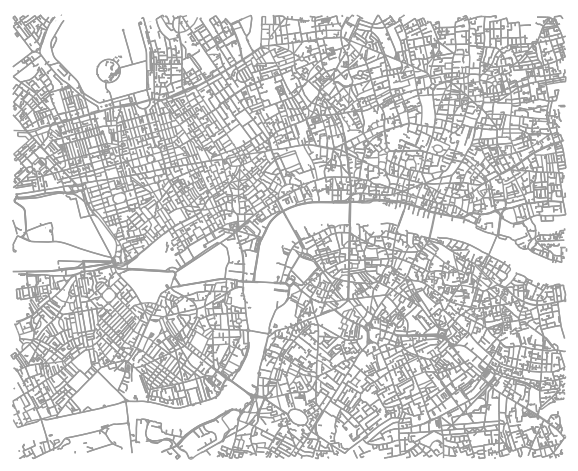
\includegraphics[width=0.5\linewidth]{bbox_bike_1_filter_cropped}
  \caption{1: most confident cyclists}
  \label{fig:sub1}
\end{figure}

\begin{figure}
  \centering
  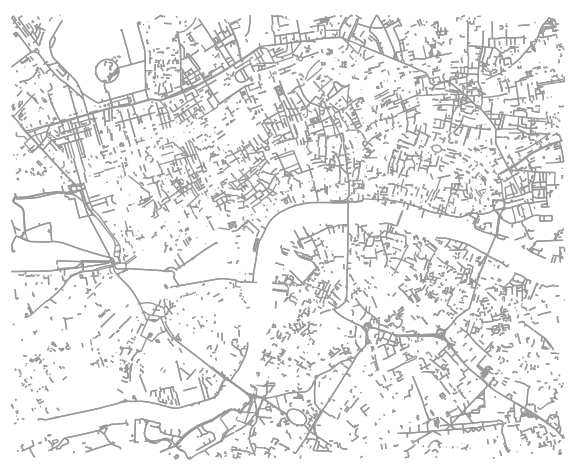
\includegraphics[width=0.5\linewidth]{bbox_bike_5_filter_cropped}
  \caption{5: no interaction with cars }
  \label{fig:sub2}
\end{figure}



\begin{figure}
  \centering
  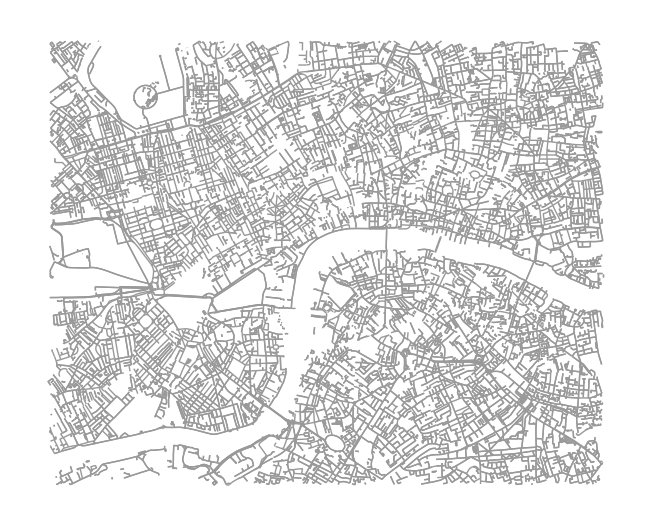
\includegraphics[width=0.5\linewidth]{bbox_bike_2_filter_cropped}
  \caption{2: all but primary and trunk streets}
  \label{fig:sub2}
\end{figure}



\begin{figure}
  \centering
  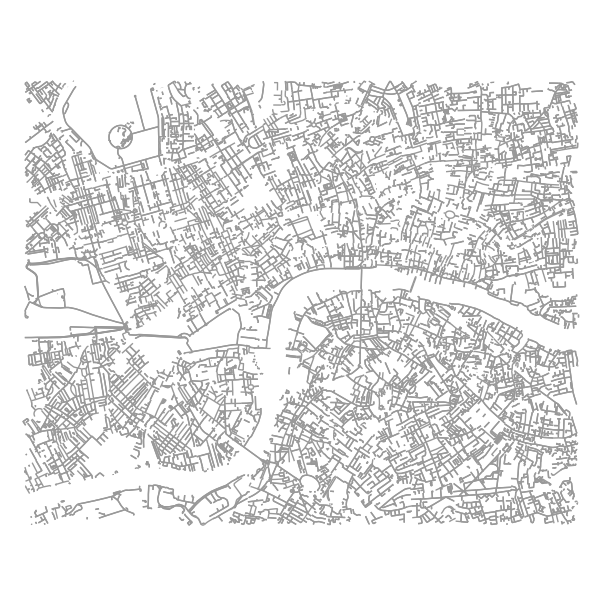
\includegraphics[width=0.5\linewidth]{bbox_bike_4_filter_cropped}
  \caption{4: only residential and living streets}
  \label{fig:sub2}
\end{figure}


\subsubsection{Quant Network}

Quant has 23,377,225 pairs. The subset has 799,236. The subset has 200,041 missing distances. 


\subsection{Network Characteristics}

chart of largest connected component of network as edge types are included. 

\begin{figure}
\centering
\caption{largest component of network type}
\label{fig:connected_component}
\end{figure}

no cars,
+ living streets
+ residential streets
+ tertiary 
+ secondary
+primary

\begin{table}
\centering
\caption{table of network statistics}
\label{table:network_stats}
\end{table}

\subsection{Defining Origins and Destinations}

Node 5816785884, closest to the centroid of LSOA XXXXXX is found at the entrance to a garage at the end of a one way street. Thus every other node in the network is inaccessible on the directed versions of the network. The edge leading to this node is tagged ``service'' so perhaps service streets should have been excluded as they are frequently dead ends. 


histogram of distances between centroid and nearest common node. 

\begin{figure}
\centering
\caption{distribution of differences between Quant distances and Cycle Origins and Destinations}
\label{fig:diff_dist}
\end{figure}

\subsection{Travel Times}

Travel times were converted from distances using a walking speed of 3 mph and a cycling speed of 8 mph based on data taken from google maps estimates for journeys as seen in that table. 


As seen table XXXXX travel times for bike network 2, without trunk or primary highways, are substantially longer than travel times for bike network 1. This indicates that the effect of removing these edges is not just to disconnect the network but also requires a network user to take a less direct route, straying further from the straight line between origin and destination. 

The difference between directed and undirected distances is also notable. 

the standard deviation 

the min is unchanged, while the max 

Travel times by bicycle for aggressive cyclists are XXXXX compared to the QUANT travel times by public transport. 

\subsubsection{test for differences}

There's got to be a significant difference between the distances for the different networks right?


\begin{table}
\centering
\caption{google speed estimates}
\label{table:google_speeds}
\end{table}


\begin{table}
\centering
\caption{travel time statistics}
\label{table:travel_time_stats}
\end{table}

\subsection{Changes in Routing}


\subsubsection{compare route across directedness}
\begin{figure}
\centering
\caption{example of routing on directed network 1}
\label{fig:routing_1}
\end{figure}

\begin{figure}
\centering
\caption{example of routing on undirected network 1}
\label{fig:routing_1}
\end{figure}

\subsubsection{compare route across level 1 and 2}

Seen in figure XXXX  compare longest path for directed network 2 to the path between those nodes in directed network 1. 

Compare longest path for directed network 1 to undirected network 1. 

compare o/d pair with largest increase in distance between directed 1 and directed 2 to the distance in undirected 2. 

Is allowing travel in any direction on side roads a good replacement for primary and trunk routes?


\begin{figure}
\centering
\caption{example of routing on directed network 1}
\label{fig:routing_1}
\end{figure}

\begin{figure}
\centering
\caption{example of routing on directed network 2}
\label{fig:routing_1}
\end{figure}

\subsubsection{compare across level 2 directedness}

\begin{figure}
\centering
\caption{example of routing on directed network 2}
\label{fig:routing_1}
\end{figure}

\begin{figure}
\centering
\caption{example of routing on undirected network 2}
\label{fig:routing_1}
\end{figure}


\subsection{Accessibility}

in qgis, color lsoa's by travel time to central lsoa. 

in QGIS color lsoa's by travel time from lsoa with highest average distance. 

in QGIS color lsoa's by  average directness, distance divided by straightline distance. 

Plot a few paths in osmnx to look at low directness. 


\begin{figure}
\centering
\caption{lsoas colored by directness of routes to other lsoas}
\label{fig:lsoa_directness}
\end{figure}

\subsection{notes on computation}


\subsection{Notes about computation}

runtimes for the distances between nodes were long. computations were done on an intel i74700HQ processor with the database contained on the internal Solid State Drive. 

Runtimes increased with the number of connected origin destination pairs, since unconnected pairs  did not require the calculation of a shortest path. Thus bike 1 travel times took longer than bike level 2. Additionally, the undirected network calculations took substantially longer than the directed networks because there were sugnificantly more route possibilities with more edges available at each node. 

Table XXXX contains calculation times by network type. 

% table for computation times across algorithm types

% table for computation times across network types
%\begin{table}[]
%\centering
%\begin{tabular}{lllll}
%network  & 1 & 1 undirected & 2  & 2 undirected   \\
%time     & 24:00   & 72:00??  & 9:03  & 36:00        \\        
%\end{tabular}
%\caption{Computation Times}
%\label{table:1}
%\end{table}

\begin{table}[]
\centering
\begin{tabular}{@{}l|llll@{}}
network     & 1           & 1 undirected & 2    & 2 undirected \\ \hline
time(hours) & $\sim$24:00 & $\sim$72:00  & 9:03 & $\sim$36:00 
\end{tabular}
\caption{Calculation times for routes}
\label{table:net_calc_times}
\end{table}

\begin{table}
\centering
\caption{computation times using different algorithms}
\label{table:comp_times_algo}
\end{table}


text


\section{Conclusions}

	% word count
% 1184


%\subsection{Key Questions}
%what was the scope and how was it defined \\ 
%what filters were used \\
%what were the walking and cycling speeds used \\
%what were the travel times calculated \\
%what was the directness of travel on different networks \\
%what is the distribution of travel times in the different networks \\
%what lsoas changed the most and least across networks \\
%how did removing road types affect the number of lsoa centers connected? \\
%how long did the calculations take? \\
%Did removing directionality from the networks have a significant effect? \\
%Did removing directionality mediate the effect of removing primary and trunk streets? \\
%


\subsection{Results}	

The primary conclusion, consistent with observation around London is that cycling on unprotected parts of high volume, main streets is a required part of moving around the city by bicycle. A high percentage of trips require the use of these types of highways. 

A reasonable representation of the London cycling network could be constructed from Open Street Map data using \texttt{OSMnx} and \texttt{Networkx}. With some specific improvements to the software and methodology a good job could be done of estimating accessibility in London by bicycle. Access to computing resources is a key consideration. The structure of the OSM data and the structure of the Overpass API query language presented some difficulty but this was essentially solvable. The largest possible problem with the construction of networks using OSM data was the potential for a complete lack of data on some feature of the street network. Given the density of the data in London this was probably not a significant concern. With the ongoing addition of the TfL Cycling Infrastructure Database OSM is probably the highest quality source for this data available today. 

There were significant regional differences in the effect of removing primary and trunk streets and those looking to improve the London cycling network may want to focus their efforts on western and northern London within the scope of the analysis. Removing direction restrictions for cyclists is probably not a good way to improve cycling safety and the directness of travel by bicycle. This did not mediate much of the change in travel times from removing primary and trunk streets. 

Compared to the conclusions of \textcite{furth2016network}, the London network did not fracture into subcomponents as the San Jose street grid did in that analysis. In the tree-like street network of London decreases in connectivity came through the complete separation of single nodes from all other nodes so that most nodes that lost connectivity with other nodes on the network were likely to lose connectivity with all other nodes. Thus while that study focused on connecting disconnected components, improvements to London's network should perhaps be targeted toward reducing trip times by improving the directness of safe routes. 

\subsection{Limitations}

Selection of origin and destination locations was an important determinant of the results. QUANT uses the transit station of highest degree as the origin and destination points, meaning that there is no walking time included in the calculation. Additionally, QUANT travel times are probabilistic in the sense that the precise start time affects the travel time because there may be a wait time for a bus or train. This is a key advantage that cycling has over public transport, a more linear relationship between distance and travel time. In one instance, the selection of a node at the end of a one way service street meant that only on the undirected networks was it connected to any other. Some LSOA's that were disconnected from the network after the removal of edges continued to contain nodes that were connected to the network. Thus the selection criteria could have a significant impact on the outcomes and could possibly be improved. 

The network representations could also be improved. \texttt{OSMnx} makes working with the Overpass API easier by abstracting away a lot of the process. Unfortunately this ease comes with a cost, a diminished ability to build an accurate network using all of the possible attributes of OSM geometries. A key feature for \texttt{OSMnx} that would improve the ability to define networks accurately would be the option to ``stack'' multiple types of requests into a full network. Collecting several sets of edges and nodes with several filters, as can be accomplished with the Overpass Turbo OSM tool \parencite{overpass_turbo}. 

It was subsequently found that Google speed estimates for cycling can vary pretty dramatically and the 13 kph speed used may be fairly conservative with subsequent tests of Google Maps speed estimates being closer to 15 kph. This does not change the overall indication of the data that public transit is faster than cycling. An empirical study of observed cycling speeds would be the optimal way to settle this question. 

Lastly, this dissertation was unable to adjust for the demand for travel between O/D pairs because of the lack of access to high resolution journey to work data. While this is unfortunate the differences in connected pairs and in average travel times between different network definitions are so large that it is highly unlikely that adjusting for relative travel demand would alter the conclusions made very meaningfully. 

\subsection{Opportunities for Improvement and Extension}

Beyond improving the implementation of the methodology used in this dissertation, the key improvement to the methodology generally would be to move from using OSM tags for highway importance, which is a discrete set of values, to a continuous estimation of the stress for a given street based on all of the possible data. As found in the section \ref{literature} review of literature, there are not clear methods for this estimation problem because of the nature of the data and difficulty of measuring cyclist volumes at a high resolution. To date no methodology has implemented a continuous estimation although \textcite{boisjoly2019bicycle} approach a basic version of this by measuring the portion of a trip completed on designated cycle infrastructure. 

While removing edges from the network did have a significant effect on connectivity, reducing the connected origin and destination pairs by 40\% the study showed that less confident cyclists have route options available to them if they are willing to go out of their way along less direct paths.

Several data sets could potentially augment this type of analysis further. London has several decades of traffic incident data with spatial data associated with an incident. This could possibly provide for validation of the high stress nature of OSM highways tagged primary and trunk. With the beginning of collection on cyclist volumes in some parts of the city, this could become possible in the future.  Additionally, high resolution journey to work data for London exists but is not publicly available due to privacy concerns. Access to this data would allow for a connectivity ratio like that of \textcite{furth2016network} that adjusts the percentage of possible trips of a reasonable length by the number of commuter trips that are associated with that origin and destination. 

"Rat-running", where traffic filters off of main routes onto side roads is a key reason that Open Street Map highway types may not have a real relationship with traffic stress or danger. A "quiet" street may get relatively more traffic than it is built to handle relative to primary routes if the quietway is a good route between destinations. This is consistent with anecdotal observations of the author that on some quiet ways traffic behavior is more dangerous and less predictable than on primary routes. It is not clear that dense slow moving traffic is more dangerous than sparse high speed traffic on back roads. If this was found to be a significant consideration in quietways it would suggest that adding "gates" that allow cyclists to pass through  but not motor vehicles may be preferable to other cycling infrastructure for improving the safety of that route. 


\pagebreak
\section{Appendix}


\pagebreak

\printbibliography

\end{document}
